% GENERATED by e2e/helpers/plot_timeline.py -- do not edit by hand.
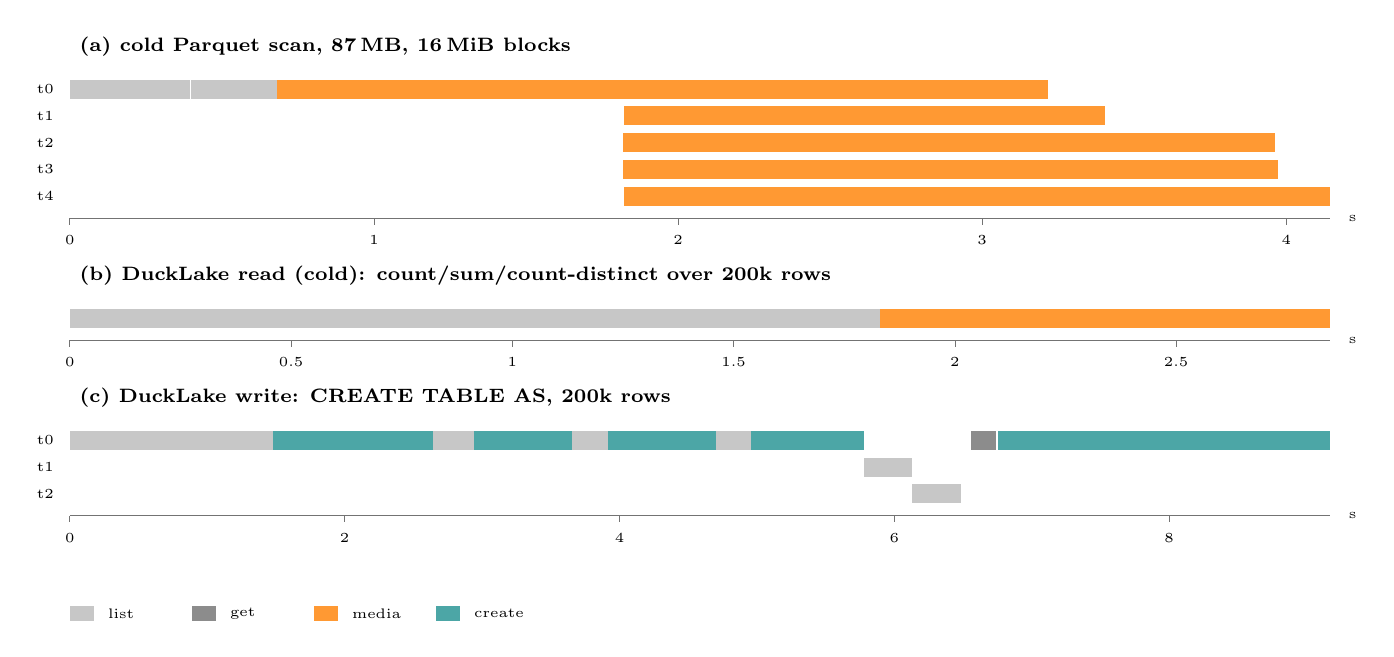
\begin{tikzpicture}[x=1cm, y=1cm]
% --- (a) cold Parquet scan, 87\,MB, 16\,MiB blocks ---
\node[anchor=west, font=\scriptsize\bfseries] at (0,0.42) {(a) cold Parquet scan, 87\,MB, 16\,MiB blocks};
\fill[black!22] (0.000,0.000) rectangle (1.531,-0.240);
\fill[black!22] (1.532,0.000) rectangle (2.632,-0.240);
\fill[orange!80] (2.633,0.000) rectangle (7.024,-0.240);
\fill[orange!80] (7.028,0.000) rectangle (12.428,-0.240);
\fill[orange!80] (7.031,-0.340) rectangle (13.151,-0.580);
\fill[orange!80] (7.029,-0.680) rectangle (15.300,-0.920);
\fill[orange!80] (7.030,-1.020) rectangle (15.344,-1.260);
\fill[orange!80] (7.031,-1.360) rectangle (16.000,-1.600);
\node[anchor=east, font=\tiny] at (-0.08,-0.120) {t0};
\node[anchor=east, font=\tiny] at (-0.08,-0.460) {t1};
\node[anchor=east, font=\tiny] at (-0.08,-0.800) {t2};
\node[anchor=east, font=\tiny] at (-0.08,-1.140) {t3};
\node[anchor=east, font=\tiny] at (-0.08,-1.480) {t4};
\draw[black!55, line width=0.3pt] (0,-1.760) -- (16.00,-1.760);
\draw[black!55, line width=0.3pt] (0.000,-1.760) -- (0.000,-1.840);
\node[anchor=north, font=\tiny] at (0.000,-1.860) {0};
\draw[black!55, line width=0.3pt] (3.862,-1.760) -- (3.862,-1.840);
\node[anchor=north, font=\tiny] at (3.862,-1.860) {1};
\draw[black!55, line width=0.3pt] (7.724,-1.760) -- (7.724,-1.840);
\node[anchor=north, font=\tiny] at (7.724,-1.860) {2};
\draw[black!55, line width=0.3pt] (11.586,-1.760) -- (11.586,-1.840);
\node[anchor=north, font=\tiny] at (11.586,-1.860) {3};
\draw[black!55, line width=0.3pt] (15.449,-1.760) -- (15.449,-1.840);
\node[anchor=north, font=\tiny] at (15.449,-1.860) {4};
\node[anchor=west, font=\tiny] at (16.12,-1.760) {s};
% --- (b) DuckLake read (cold): count/sum/count-distinct over 200k rows ---
\node[anchor=west, font=\scriptsize\bfseries] at (0,-2.49) {(b) DuckLake read (cold): count/sum/count-distinct over 200k rows};
\fill[black!22] (0.000,-2.910) rectangle (1.926,-3.150);
\fill[black!22] (1.927,-2.910) rectangle (4.213,-3.150);
\fill[black!22] (4.213,-2.910) rectangle (5.739,-3.150);
\fill[black!22] (5.739,-2.910) rectangle (7.203,-3.150);
\fill[black!22] (7.203,-2.910) rectangle (8.854,-3.150);
\fill[black!22] (8.854,-2.910) rectangle (10.293,-3.150);
\fill[orange!80] (10.294,-2.910) rectangle (16.000,-3.150);
\draw[black!55, line width=0.3pt] (0,-3.310) -- (16.00,-3.310);
\draw[black!55, line width=0.3pt] (0.000,-3.310) -- (0.000,-3.390);
\node[anchor=north, font=\tiny] at (0.000,-3.410) {0};
\draw[black!55, line width=0.3pt] (2.810,-3.310) -- (2.810,-3.390);
\node[anchor=north, font=\tiny] at (2.810,-3.410) {0.5};
\draw[black!55, line width=0.3pt] (5.620,-3.310) -- (5.620,-3.390);
\node[anchor=north, font=\tiny] at (5.620,-3.410) {1};
\draw[black!55, line width=0.3pt] (8.430,-3.310) -- (8.430,-3.390);
\node[anchor=north, font=\tiny] at (8.430,-3.410) {1.5};
\draw[black!55, line width=0.3pt] (11.240,-3.310) -- (11.240,-3.390);
\node[anchor=north, font=\tiny] at (11.240,-3.410) {2};
\draw[black!55, line width=0.3pt] (14.050,-3.310) -- (14.050,-3.390);
\node[anchor=north, font=\tiny] at (14.050,-3.410) {2.5};
\node[anchor=west, font=\tiny] at (16.12,-3.310) {s};
% --- (c) DuckLake write: CREATE TABLE AS, 200k rows ---
\node[anchor=west, font=\scriptsize\bfseries] at (0,-4.04) {(c) DuckLake write: CREATE TABLE AS, 200k rows};
\fill[black!22] (0.000,-4.460) rectangle (0.707,-4.700);
\fill[black!22] (0.707,-4.460) rectangle (1.182,-4.700);
\fill[black!22] (1.182,-4.460) rectangle (1.658,-4.700);
\fill[black!22] (1.658,-4.460) rectangle (2.140,-4.700);
\fill[black!22] (2.140,-4.460) rectangle (2.577,-4.700);
\fill[teal!70] (2.578,-4.460) rectangle (4.606,-4.700);
\fill[black!22] (4.606,-4.460) rectangle (5.126,-4.700);
\fill[teal!70] (5.126,-4.460) rectangle (6.378,-4.700);
\fill[black!22] (6.378,-4.460) rectangle (6.840,-4.700);
\fill[teal!70] (6.840,-4.460) rectangle (8.210,-4.700);
\fill[black!22] (8.210,-4.460) rectangle (8.655,-4.700);
\fill[teal!70] (8.655,-4.460) rectangle (10.081,-4.700);
\fill[black!22] (10.081,-4.800) rectangle (10.689,-5.040);
\fill[black!22] (10.691,-5.140) rectangle (11.314,-5.380);
\fill[black!45] (11.449,-4.460) rectangle (11.766,-4.700);
\fill[teal!70] (11.782,-4.460) rectangle (16.000,-4.700);
\node[anchor=east, font=\tiny] at (-0.08,-4.580) {t0};
\node[anchor=east, font=\tiny] at (-0.08,-4.920) {t1};
\node[anchor=east, font=\tiny] at (-0.08,-5.260) {t2};
\draw[black!55, line width=0.3pt] (0,-5.540) -- (16.00,-5.540);
\draw[black!55, line width=0.3pt] (0.000,-5.540) -- (0.000,-5.620);
\node[anchor=north, font=\tiny] at (0.000,-5.640) {0};
\draw[black!55, line width=0.3pt] (3.490,-5.540) -- (3.490,-5.620);
\node[anchor=north, font=\tiny] at (3.490,-5.640) {2};
\draw[black!55, line width=0.3pt] (6.980,-5.540) -- (6.980,-5.620);
\node[anchor=north, font=\tiny] at (6.980,-5.640) {4};
\draw[black!55, line width=0.3pt] (10.470,-5.540) -- (10.470,-5.620);
\node[anchor=north, font=\tiny] at (10.470,-5.640) {6};
\draw[black!55, line width=0.3pt] (13.960,-5.540) -- (13.960,-5.620);
\node[anchor=north, font=\tiny] at (13.960,-5.640) {8};
\node[anchor=west, font=\tiny] at (16.12,-5.540) {s};
\fill[black!22] (0.00,-6.69) rectangle (0.30,-6.87);
\node[anchor=west, font=\tiny] at (0.36,-6.78) {list};
\fill[black!45] (1.55,-6.69) rectangle (1.85,-6.87);
\node[anchor=west, font=\tiny] at (1.91,-6.78) {get};
\fill[orange!80] (3.10,-6.69) rectangle (3.40,-6.87);
\node[anchor=west, font=\tiny] at (3.46,-6.78) {media};
\fill[teal!70] (4.65,-6.69) rectangle (4.95,-6.87);
\node[anchor=west, font=\tiny] at (5.01,-6.78) {create};
\end{tikzpicture}
